\section{Bootstrapping}

\subsection{a)}
\begin{figure}[H]
    \centering
    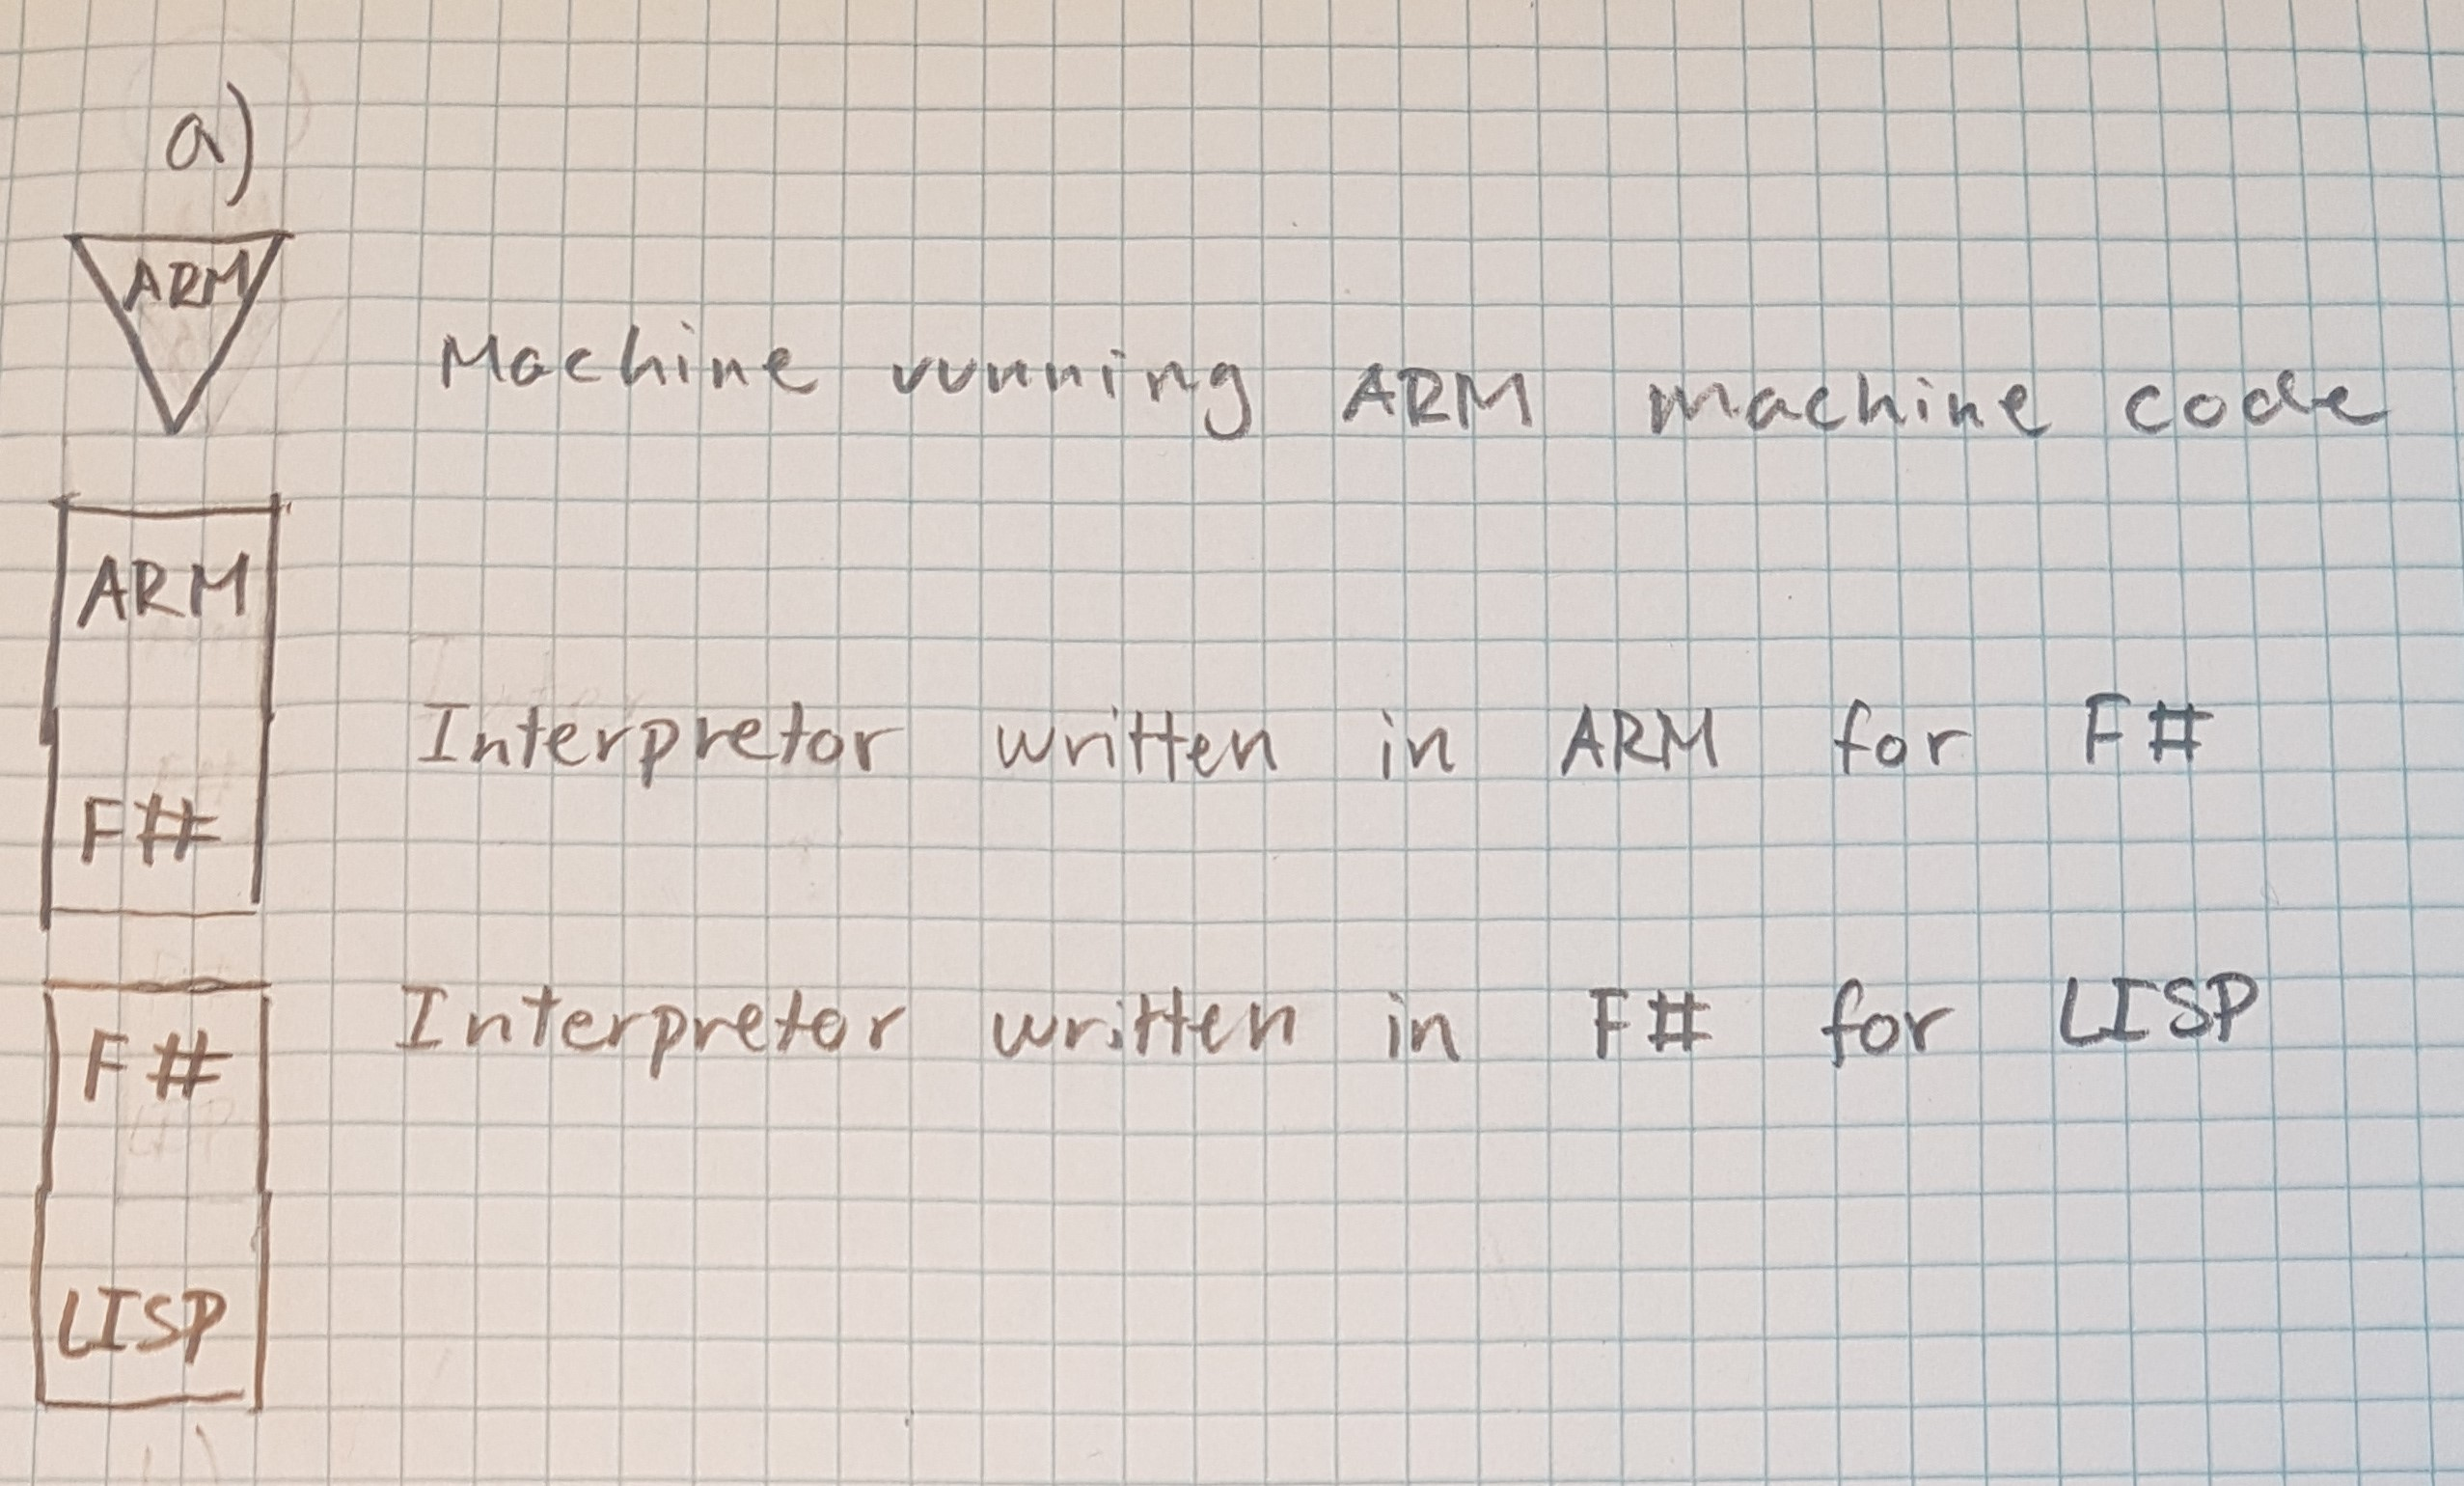
\includegraphics[width=0.75\textwidth]{Figures/PLD_A1_Q3_A_cropped.jpg}
    \caption{Bratman diagrams for the components}
\end{figure}

\subsection{b)}

\begin{figure}[H]
    \centering
    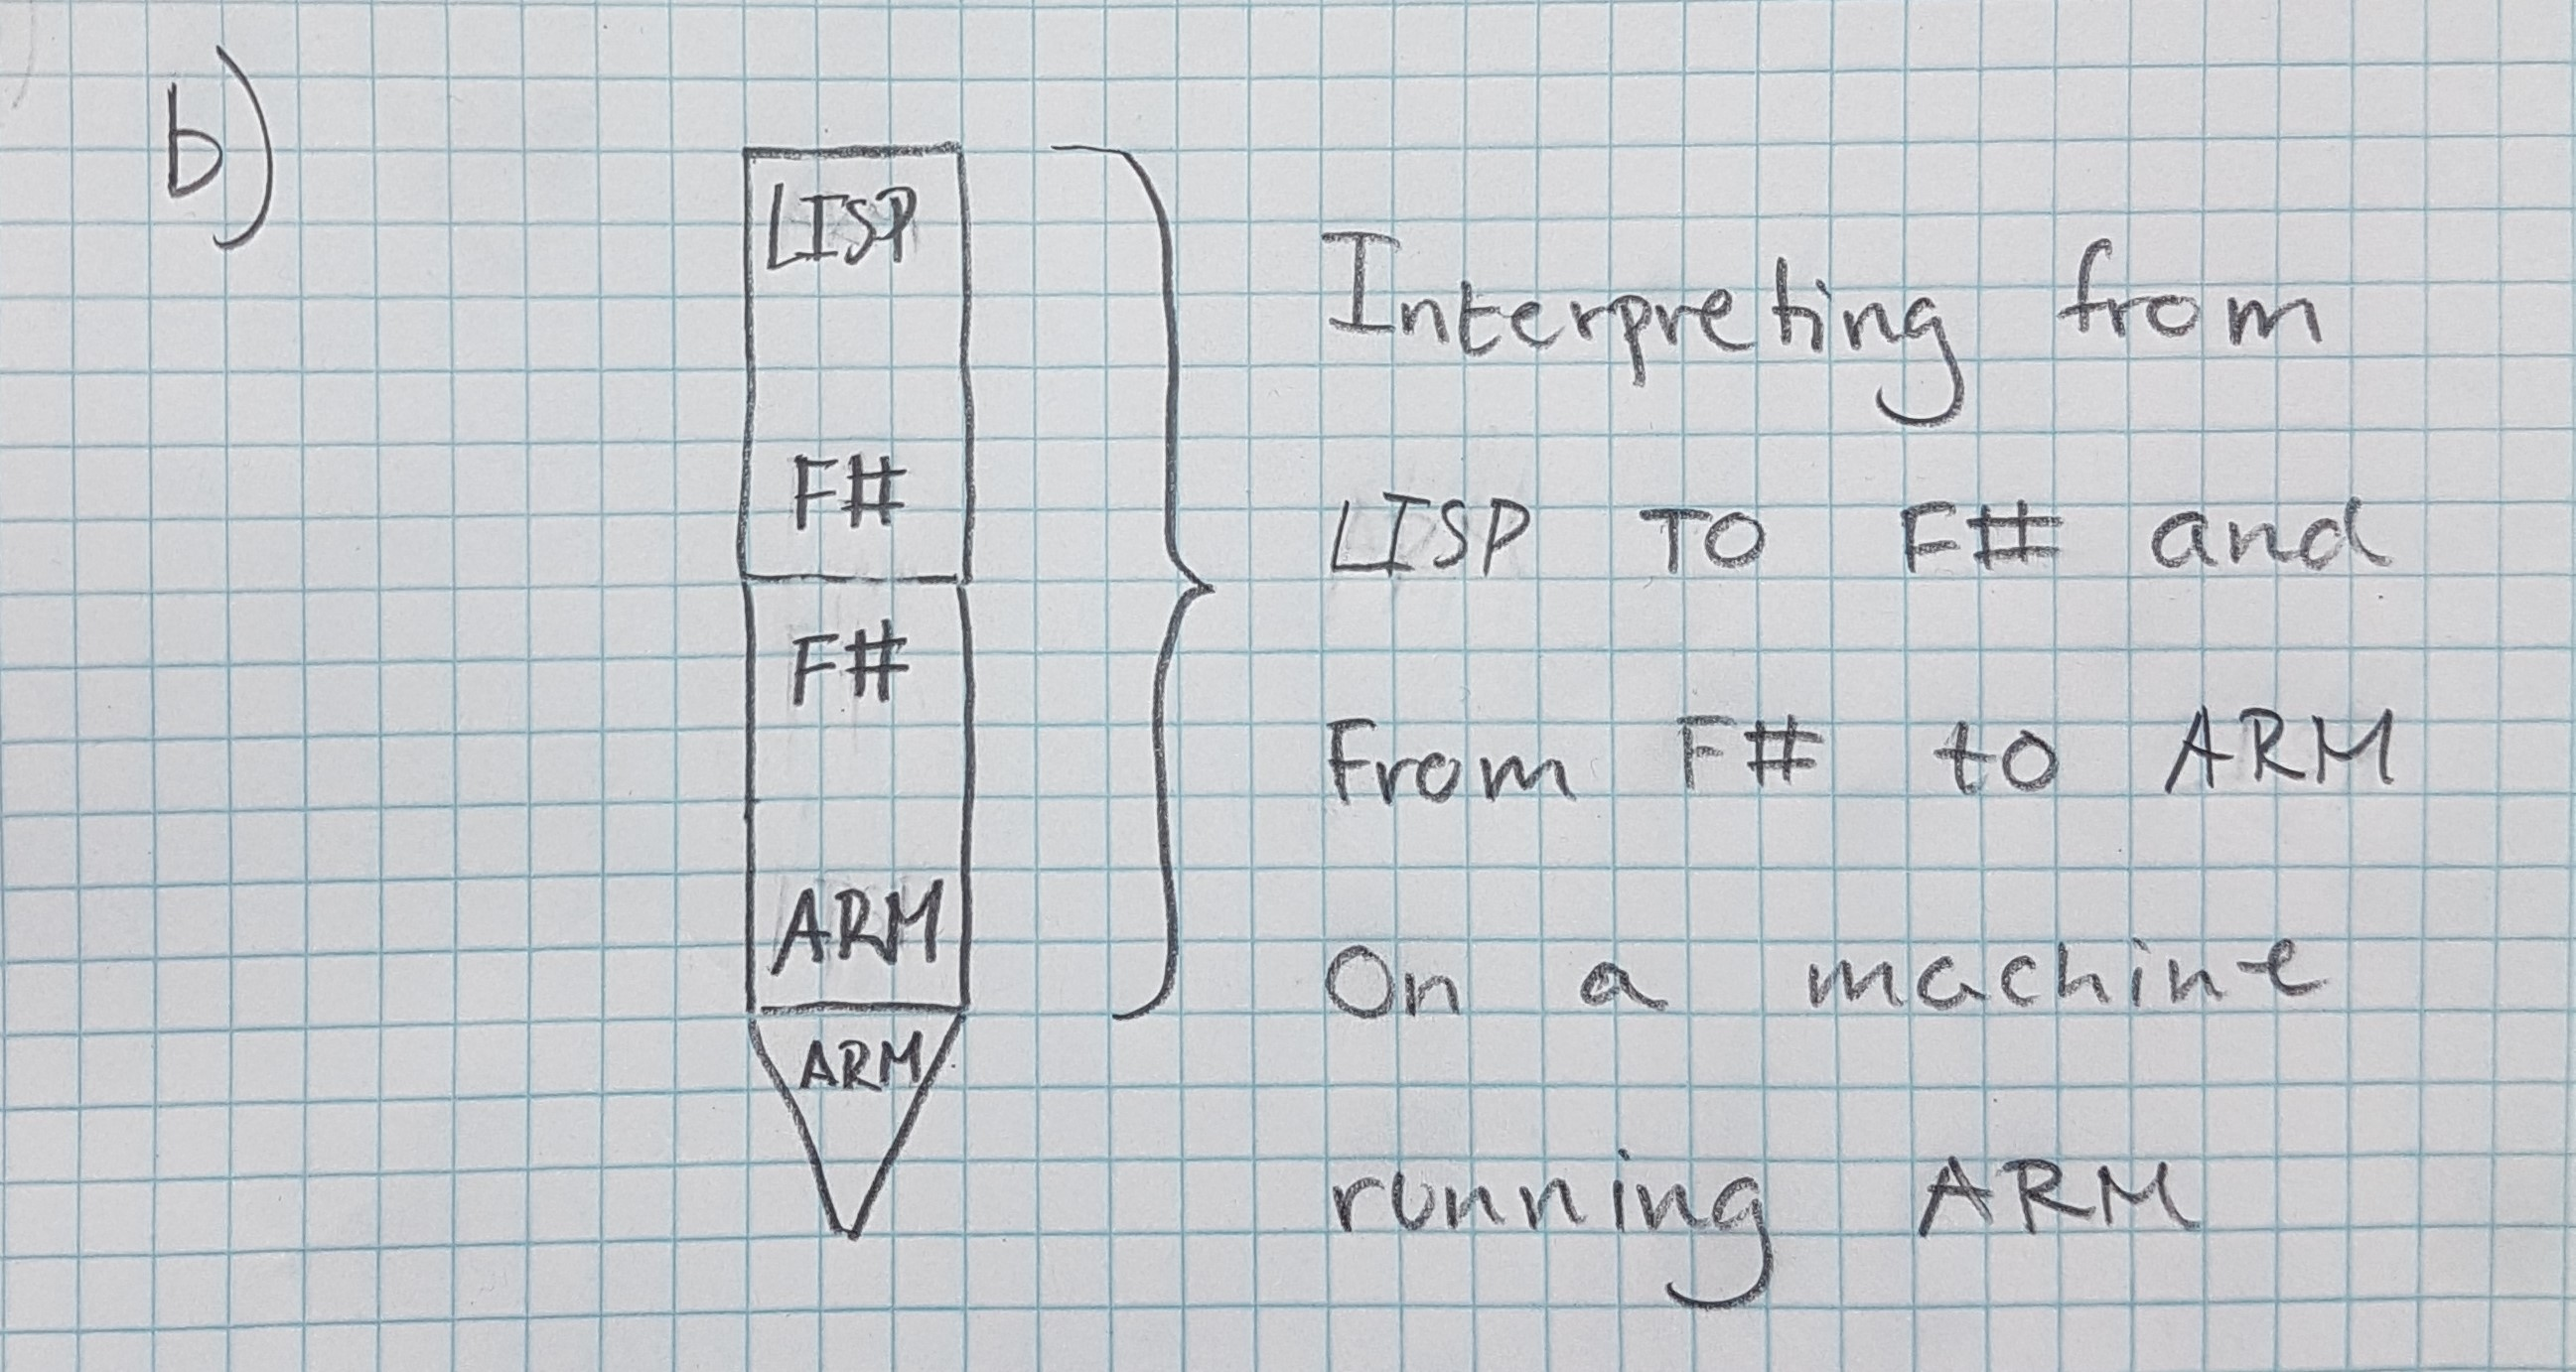
\includegraphics[width=0.75\textwidth]{Figures/PLD_A1_Q3_B_cropped.jpg}
    \caption{Bratman diagram for executing a LISP program}
\end{figure}

I would argue it's not possible to execute a program in LISP with the following components, unless you're allowred to rearrange the way the
interpreters are setup and create a "new" interpreter that interpret from LISP $\rightarrow$ ARM.
\\
\\
meaning you interpret from:
\\
ARM $\rightarrow$ F\# $\rightarrow$ F\# $\rightarrow$ LISP $\rightarrow$ LISP $\rightarrow$ ARM $\xrightarrow[]{\text{execute}}$ ARM-machine 